\section{DeepEMhancer Sharpening protocol}
\label{app:deepEMhancerSharpening}%a103

Protocol designed to apply $DeepEMhancer$, the automatic map postprocessing method that sharpens and maks part of the noise at medium/high resolution \citep{Sanchez-Garcia2020.06.12.148296}, in \scipion. Detailed information of this method can be also obtained in \url{https://github.com/rsanchezgarc/deepEMhancer}.

\begin{itemize}
 \item Requirements to run this protocol and visualize results:
    \begin{itemize}
        \item \scipion plugin: \ttt{scipion-em-xmipp}
        \item \scipion plugin: \ttt{scipion-em-chimera}
    \end{itemize}
 \item \scipion menu:\\
  \ttt{Model building -> Preprocess map} (\ffigure{fig:app_deepEMhancer_1} (A))
  
 \item Protocol form parameters (\ffigure{fig:app_deepEMhancer_1} (B)):
  
    \begin{figure}[H]
     \centering 
     \captionsetup{width=.7\linewidth} 
     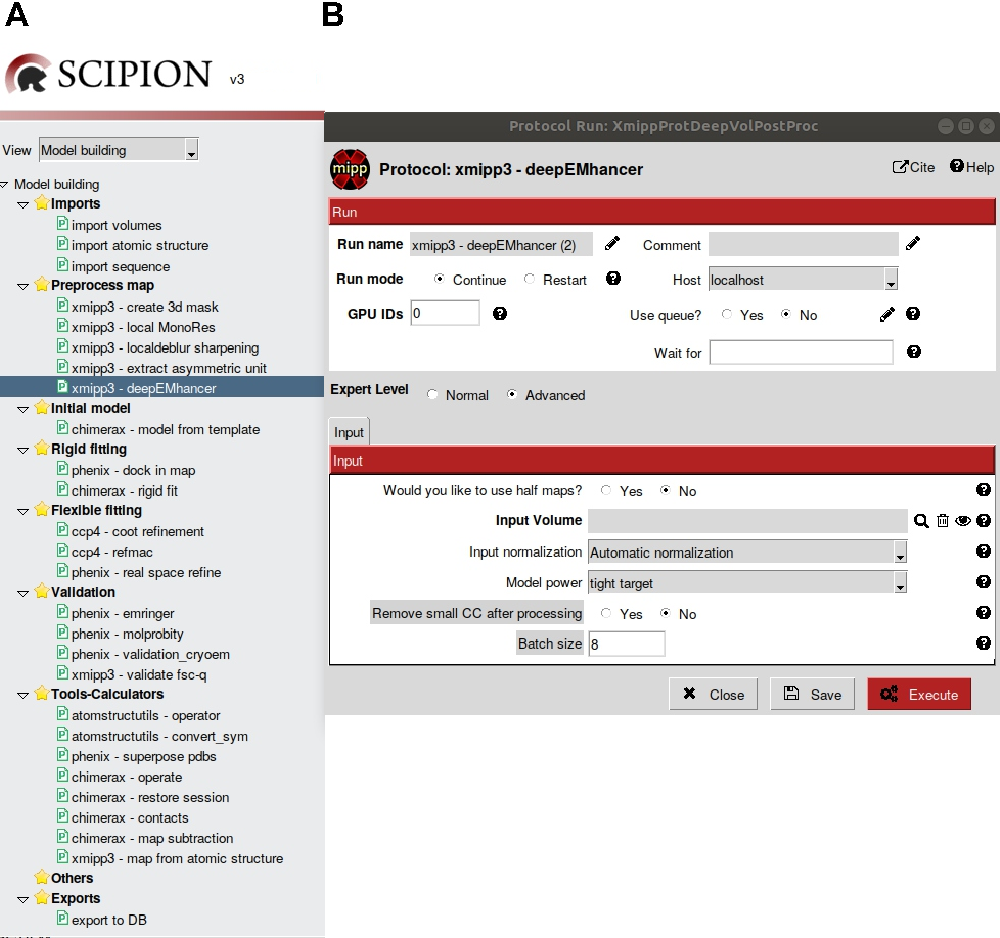
\includegraphics[width=0.90\textwidth]{Images_appendix/Fig303}
     \caption{Protocol \scommand{xmipp3 - deepEMhancer}. A: Protocol location in \scipion menu. B: Protocol form.}
     \label{fig:app_deepEMhancer_1}
    \end{figure}
    
    \begin{itemize}
        \item \ttt{Would you like to use half maps?}: Although the result will be the same if you decide to use half maps or a non-sharpened non-masked map, a way to ensure that you have selected the right input map is providing half maps. In addition, the algorithm has been trained with half maps. The first step performed by the protocol is to compute the average map. Then, select \ttt{Yes} whenever you can provide half maps, otherwise be sure you have the right average map, usually generated during the reconstruction by map refinement. However, the algorithm does not work correctly using post-processed maps. Since the two half maps can be obtained directly as independent maps or being associated to the average map, if you select \ttt{Yes} a new question will appear:
            \begin{itemize}
            \item \ttt{Are the half maps included in the volume?}: Select \ttt{Yes} if your input average map has the two half maps associated. If this is the case, complete the next form param. Otherwise, you should provide both half maps as independent preexisting \scipion objects. To add those half maps a couple of form params will apper to fill in with each half map:
                \begin{itemize}
                \item \ttt{Volume Half 1}
                \item \ttt{Volume Half 2}
                \end{itemize}
            \end{itemize}
        \item \ttt{Input Volume}: Unsharpened unmasked electron density map previously downloaded or generated in \scipion.
        \item \ttt{Input normalization}: We need apply normalization to accomodate the intensity values of map to the specific range of values of the trained neural network. Three possible normalization methods are suggested:
        \begin{itemize}
            \item \ttt{Automatic normalization}: Default normalization mode that forces the noise average to be zero and the standard deviation 0.1 in an spheric shell around the specimen. Since then the noise always displays a similar distribution, the network gets easier to distinguish noise from signal. This method usually works correctly in almost any case. Exceptions could be very long specimens (fiber proteins) or those having big empty spaces (big viruses).
            \item \ttt{Normalization from statistics}: Similar to the first one although in this case users provide their own statistics of noise average and standard deviation.
            \item \ttt{Normalization from binary mask}
        \end{itemize}
        
        \item \ttt{Resolution Map}: Resolution map generated by protocols like \scommand{xmipp3 - local MonoRes}. The resolution value in the corresponding voxel of the \ttt{Input map} is assigned to each voxel of the \ttt{Resolution Map}.
        \item \ttt{lambda}: Since $LocalDeblur$ is based on an iterative formula repeated until a convergence criterion is reached, \ttt{$lambda$} is the step size advanced parameter that modulates the speed of convergence. The default value, \ttt{$lambda$} = 1, indicates that the method itself establishes automatically the value of \ttt{$lambda$}. Although the default value is small enough to guarantee the convergence and large enough to speed it up, the \ttt{$lambda$} value can be increased by the user to accelerate the convergence process. Unlike the default value, that grows along the convergence process, the \ttt{$lambda$} value selected by the user will be maintained constant. Falling into a local minimum is a risk derived of increasing the convergence speed.
        \item \ttt{K}: Weight assigned to the difference between the local resolution and the spatial frequency of the center of each bandpass filter. This difference weighted by \ttt{K} is the base to compute the local weight of each channel in the filter bank, that correlates the input map with the sharpened map. The bigger the value of \ttt{K}, the lower the weight of each channel in the filter bank. Maximum weights are obtained when local resolution and spatial frequency of the center of each bandpass filter show identical values.
    \end{itemize}
    
    \item Protocol execution:\\
  Adding specific map/structure label is recommended in \ttt{Run name} section, at the form top. To add the label, open the protocol form, press the pencil symbol at the right side of \ttt{Run name} box, complete the label in the new opened window, press OK and, finally, close the protocol. This label will be shown in the output summary content (see below). If you want to run again this protocol, do not forget to set to \ttt{Restart} the \ttt{Run mode}.\\
  Press the \ttt{Execute} red button at the form bottom.
  
  \item Visualization of protocol results:
  
  After executing the protocol, press \ttt{Analyze Results} and a menu window will be opened with $ShowJ$ (\url{https://github.com/I2PC/scipion/wiki/ShowJ}), the default \scipion viewer, including the maps generated in each independent iteration before getting convergence. The sharpening algorithm stops when the difference between two successive iterations is lower than 1\%, thus generating variable number of maps before stopping. The $ShowJ$ window menu (\ttt{File -> Open with Chimera}) allows to open the selected map in $Chimera$ graphics window.
  
  \item Summary content:
  \begin{itemize}
     \item Protocol output (below \scipion framework):\\ \ttt{xmipp3 - localdeblur sharpening -> ouputVolumes}; SetOfVolumes (number of items, x, y, and z dimensions, sampling rate).
     \item \ttt{SUMMARY} box:\\ \ttt{LocalDeblur Map}.
  \end{itemize}
    
\end{itemize}

